\documentclass[letterpaper,12pt,oneside]{article}\usepackage[]{graphicx}\usepackage[]{color}
%% maxwidth is the original width if it is less than linewidth
%% otherwise use linewidth (to make sure the graphics do not exceed the margin)
\makeatletter
\def\maxwidth{ %
  \ifdim\Gin@nat@width>\linewidth
    \linewidth
  \else
    \Gin@nat@width
  \fi
}
\makeatother

\definecolor{fgcolor}{rgb}{0.345, 0.345, 0.345}
\newcommand{\hlnum}[1]{\textcolor[rgb]{0.686,0.059,0.569}{#1}}%
\newcommand{\hlstr}[1]{\textcolor[rgb]{0.192,0.494,0.8}{#1}}%
\newcommand{\hlcom}[1]{\textcolor[rgb]{0.678,0.584,0.686}{\textit{#1}}}%
\newcommand{\hlopt}[1]{\textcolor[rgb]{0,0,0}{#1}}%
\newcommand{\hlstd}[1]{\textcolor[rgb]{0.345,0.345,0.345}{#1}}%
\newcommand{\hlkwa}[1]{\textcolor[rgb]{0.161,0.373,0.58}{\textbf{#1}}}%
\newcommand{\hlkwb}[1]{\textcolor[rgb]{0.69,0.353,0.396}{#1}}%
\newcommand{\hlkwc}[1]{\textcolor[rgb]{0.333,0.667,0.333}{#1}}%
\newcommand{\hlkwd}[1]{\textcolor[rgb]{0.737,0.353,0.396}{\textbf{#1}}}%

\usepackage{framed}
\makeatletter
\newenvironment{kframe}{%
 \def\at@end@of@kframe{}%
 \ifinner\ifhmode%
  \def\at@end@of@kframe{\end{minipage}}%
  \begin{minipage}{\columnwidth}%
 \fi\fi%
 \def\FrameCommand##1{\hskip\@totalleftmargin \hskip-\fboxsep
 \colorbox{shadecolor}{##1}\hskip-\fboxsep
     % There is no \\@totalrightmargin, so:
     \hskip-\linewidth \hskip-\@totalleftmargin \hskip\columnwidth}%
 \MakeFramed {\advance\hsize-\width
   \@totalleftmargin\z@ \linewidth\hsize
   \@setminipage}}%
 {\par\unskip\endMakeFramed%
 \at@end@of@kframe}
\makeatother

\definecolor{shadecolor}{rgb}{.97, .97, .97}
\definecolor{messagecolor}{rgb}{0, 0, 0}
\definecolor{warningcolor}{rgb}{1, 0, 1}
\definecolor{errorcolor}{rgb}{1, 0, 0}
\newenvironment{knitrout}{}{} % an empty environment to be redefined in TeX

\usepackage{alltt}
\usepackage[paperwidth=8.5in,paperheight=11in,top=1in,bottom=1in,left=1in,right=1in]{geometry}
\usepackage{setspace}
\usepackage[colorlinks=true,allcolors=Blue]{hyperref}
\usepackage[usenames,dvipsnames]{xcolor}
\usepackage{indentfirst}
\usepackage{titlesec}
\usepackage{multirow}
\usepackage{booktabs}
\usepackage{graphicx}
\usepackage{verbatim}
\usepackage{rotating}
\usepackage{tabularx}
\usepackage{outlines}
\usepackage{lineno}
\usepackage{array}
\usepackage{times}
\usepackage{cleveref}
\usepackage{acronym}
\usepackage[position=t]{subfig}
\usepackage{paralist}
\usepackage[noae]{Sweave}
\usepackage{natbib}
\usepackage{array}
\usepackage{pdflscape}
\usepackage{bm}
\usepackage{showlabels}
\bibpunct{(}{)}{,}{a}{}{,}

% page margins and section title formatting
\linespread{2}
\setlength{\footskip}{0.5in}
\titleformat*{\section}{\Large\bf\em}
\titleformat*{\subsection}{\singlespace\large\bf}
\titleformat*{\subsubsection}{\singlespace\normalsize\bf\em}
\titlespacing{\section}{0in}{0in}{0in}
\titlespacing{\subsection}{0in}{0in}{0in}
\titlespacing{\subsubsection}{0in}{0in}{0in}

% cleveref options
\crefname{table}{Table}{Tables}
\crefname{figure}{Fig.}{Figs.}
\renewcommand{\figurename}{Fig.}

% aliased citations
\defcitealias{CDMO14}{CDMO 2014}
\defcitealias{RDCT14}{RDCT 2014}

% acronyms
\acrodef{DO}[DO]{dissolved oxygen}
\acrodef{NERRS}[NERRS]{National Estuarine Research Reserve System}
\acrodef{RMSE}[RMSE]{root mean square error}
\acrodef{SWMP}[SWMP]{System Wide Monitoring Program}
\acrodef{WRTDS}[WRTDS]{weighted regression on time, discharge, and season}

% assorted functions
% for multiple rows in table headers
\newcommand{\head}[2]{\multicolumn{1}{>{\arraybackslash}p{#1}}{#2}}
% for milligrams per litre
\newcommand{\mgl}{mg L$^{-1}$}

% hides (not removes) numbering for section, subsection, etc.
% left indents
\renewcommand{\thesection}{}
\renewcommand{\thesubsection}{}
\renewcommand{\thesubsubsection}{}
\makeatletter
\def\@seccntformat#1{\csname #1ignore\expandafter\endcsname\csname the#1\endcsname\quad}
\let\sectionignore\@gobbletwo
\def\@subseccntformat#1{\csname #1ignore\expandafter\endcsname\csname the#1\endcsname\quad}
\let\subsectionignore\@gobbletwo
\def\@subsubseccntformat#1{\csname #1ignore\expandafter\endcsname\csname the#1\endcsname\quad}
\let\subsubsectionignore\@gobbletwo
\let\latex@numberline\numberline
\def\numberline#1{\if\relax#1\relax\else\latex@numberline{#1}\fi}
\makeatother

%knitr options


% dependent data



\IfFileExists{upquote.sty}{\usepackage{upquote}}{}
\begin{document}

\raggedbottom
% \linenumbers
\raggedright
\urlstyle{same}
\setlength{\parindent}{0.5in}
\renewcommand\refname{References \vspace{12pt}}

%%%%%%
% title page
\begin{singlespace}
\title{{\bf {\Large Improving estimates of ecosystem metabolism by removing effects of tidal advection in dissolved oxygen time series}}}
\author{
  {\bf {\normalsize Marcus W. Beck$^1$, Michael C. Murrell$^2$, James D. Hagy III$^2$}}
  \\\\{\textit {\normalsize $^1$ORISE Research Participation Program}}
  \\{\textit {\normalsize USEPA National Health and Environmental Effects Research Laboratory}}
	\\{\textit {\normalsize Gulf Ecology Division, 1 Sabine Island Drive, Gulf Breeze, FL 32561}}
	\\{\textit {\normalsize Phone: 850-934-2480, Fax: 850-934-2401, Email: \href{mailto:beck.marcus@epa.gov}{beck.marcus@epa.gov}}}
  \\\\{\textit {\normalsize $^2$USEPA National Health and Environmental Effects Research Laboratory}}
	\\{\textit {\normalsize Gulf Ecology Division, 1 Sabine Island Drive, Gulf Breeze, FL 32561}}
	\\{\textit {\normalsize Phone: 850-934-2433, Fax: 850-934-2401, Email: \href{mailto:murrell.michael@epa.gov}{murrell.michael@epa.gov}}}
  \\\\{\textit {\normalsize $^3$USEPA National Health and Environmental Effects Research Laboratory}}
	\\{\textit {\normalsize Gulf Ecology Division, 1 Sabine Island Drive, Gulf Breeze, FL 32561}}
	\\{\textit {\normalsize Phone: 850-934-2455, Fax: 850-934-2401, Email: \href{mailto:hagy.jim@epa.gov}{hagy.jim@epa.gov}}}
	}
\date{}
\maketitle
\vfill{\centerline{\textit {\normalsize Running head: Improving Estimates of Estuary Metabolism}}}
\end{singlespace}
\clearpage

%%%%%%
% acknowledgments
\section{Acknowledgments}

%%%%%%
% abstract
\centerline{{\bf Abstract}}
\begin{singlespace} \small
\noindent 
Reliable estimates of ecosystem metabolism depend on measures of \ac{DO} flux that are dominated by biological processes.  Long-term time series of \ac{DO} measurements may include variation related to both biological and physical processses such that the use of observed data may be insufficient or even misleading in some examples.  Statistical modelling techniques that dynamically quantify variation in \ac{DO} over time and tidal changes have the potential to isolate biological signals in \ac{DO} variation to more accurately estimate metabolism.  A weighted regression method that estimates \ac{DO} as a function of time and tidal height was developed to normalize, or detide, the predicted \ac{DO} signal to remove the influence of physical advection on metabolism estimates.  First, a simulation approach was used to create multiple \ac{DO} time series with known additive components of biological and physical variation on different periods.  Comparisons of detided estimates with the known, simulated biological component of the \ac{DO} signal suggested the method accurately and precisely removed varation attributed to tidal advection.  Extension of the method to four case studies provided a proof of concept illustrating the method could be useful for real-world applications. We provide a detailed discussion on use of the method for improving certainty in evaluation of \ac{DO} measurements from sites with strong tidal influences.  Moreover, we propose that the method could expand use of the open-water method for estimating ecosystem metaoblism in estuaries given that the approach can produce robust estimates of \ac{DO} values that are independent of tidal advection.  In particular, this could facilitate the use of shorter deployment periods for water quality monitors or incomplete time series given that known biases related to water movement could be removed with weighted regression. 
\normalsize
\end{singlespace}
\noindent {\bf Key words}:

\acresetall
\clearpage

%%%%%%
% intro
\section{Introduction} \label{intro}

Ecosystem metabolism is broadly defined as the difference between primary production and aerobic respiration and provides a basis for evaluating trophic state \citep{Kemp12,Needoba12}.  Primary producers, such as phytoplankton, establish the means of energy transfer to upper trophic levels. Productive systems are characterized by more efficient transfer of organic matter between trophic levels, whereas less productive systems are sinks of organic matter that are supported by allochthonous sources of energy input.  The balance between production and respiration is an integrated measure of metabolism that accounts for varying rates in processes that create and consume organic matter.  Although metabolic rates vary naturally in different regions \citep{Caffrey04}, human activities and infrastructure development are contributing factors that increase rates of production \citep{Diaz08}.  Inputs of limiting nutrients beyond background concentrations may decrease the resilience of an ecosystem such that higher rates of production are coupled with higher biological oxygen demand \citep{Yin04,Kemp09}.  Cultural eutrophication is frequently linked to declines in water quality through lower levels of dissolved oxygen and increased frequency of noxious algal blooms.  Reliables estimates of ecosystem metabolism are critical for measuring both background rates of production and potential impacts of human activities on ecosytem condition.     

Ecosystem metabolism can be estimated using several techniques, each of which is appropriate under different conditions or assumptions.   Bottle-based techniques rely on rate measurements from discrete water quality samples, whereas open-water techniques infer metabolic rates using \textit{in situ} measurements from continuous monitoring data.  Bottle-based techniques are useful for direct partitioning of metabolic contributions into discrete habitats, such as planktonic production rates during specific time periods \citep{Kemp12}.  However, such measurements may be inappropriate for evaluating whole ecosystem metabolism if significant production occurs in habitats that are not sampled, such as benthic or seagrass production.  As such, the open-water technique provides an integrative measure of metabolism by inferring process rates from \textit{in situ}, continuous monitoring data.  Originally proposed for use in streams \citep{Odum56}, the method has been used with varying success in lakes \citep{Staehr10,Coloso11,Batt12} and estuaries \citep{Caffrey04,Hopkinson05,Caffrey13}.  The ability of the open-water method to accurately estimate metabolism depends on whether the assumptions for its use are met, which are often only implicity verified in practiced. 

The open-water method uses the diel fluctuation of dissolved oxygen to infer rates of ecosytem metabolism, after correcting for losses or gains through air-water exchange \citep{Kemp12}.  Daily integrated measurements of metabolism are based on the balance between daytime estimates of gross production and nighttime estimates of respiration extrapolated to a 24 hour period.  The fundamental assumption of the open-water method is that measurements come from a water mass that has the same recent history \citep{Needoba12}.  Estimates of metabolism from a single location may be inaccurate if substantial variation in water column mixing occurs throughout the period of observation.  As such, the original technique designed for use in streams requires the comparison of data from an upstream and downstream station \citep{Odum56}.  Application of the method to systems without continuous flow, such as lakes or estuaries, have often assumed that a single sampling station provides sufficient data for estimating metabolism \cite{Staehr10}.  While single stations may be valid under specific conditions, numerous studies have shown that the open-water method may be inappropriate given the effects of physical mixing \citep{Ziegler98,Caffrey03,Coloso11,Batt12,Nidzieko14}.

The open-water method has recently been applied to coastal and oceanic ecosystems with mixed success.  An exhaustive analysis by \citet{Caffrey03} applied the method to estimate metabolim at 28 continuous monitoring stations at 14 US estuaries.  Data from two of the reserves were used to evaluate the assumption of homogeneity of water masses measured by each sensor.  Although significant differences were not observed for metabolism estimates between adjacent stations, the analysis was based on a comparison of means using conventional significance tests rather than a systematic comparison of time series.  Moreover, a portion of metabolism estimates from all stations were negative for production during the day and positive for respiration during the night.  These values were opposite in sign than expected since production increases oxygen during the day (i.e., positive effect on metabolism) and respiration consumes oxygen at night (i.e., negative effect on metabolism).  These `anamolous' values were attributed to violations in the assumption of water-column heterogeneity.  Specifically, tidal variation could have caused sampling of different water masses by individual water quality sondes as water moved inland or seaward with changing tide. 

The effects of tidal advection on estimates of ecosystem metabolism have been a point of concern in numerous studies \citep{Ziegler98,Caffrey03,Collins13,Howarth14}, although systematic estimates of its effects and methods for accounting for physical variation in \ac{DO} measurements have been minimal.  An exception is presented by \citet{Nidzieko14} through quantitative assessment of the effects of fortnightly tidal modulations on metabolism estimates.  Using a control volume approach to measure fluxes into and out of a shallow tidal creek, significant biases in metabolism estimates were observed.  Net heterotrophy was observed during spring tides, whereas metabolism was balanced during neap tides.  The timing of irradiance relative to the tidal cycle was a primary factor contributing to heterotrophy during summer months such that maximum tides occurred during the night, increasing total area for respiration.  The results of the analysis, although specific to the study location, suggest that the effects of tidal advection on \ac{DO} measurements are of primary concern when selecting locations and length of time for sonde deployment in estuaries.  In many cases, the relative magnitude of these effects may be a significant source of bias without quantitative evaluation to determine the roles of biological and physical signals in \ac{DO} measurements. Analytical techniques to evaluate and correct for tidal advection could improve certainty in metabolism estimates and also increase the use of data from shorter deployment periods if sources of bias are quantified and removed.       

This article describes use of a novel method for quantifying and removing noise in estimates of ecosystem metabolim for estuaries.  Specifically, we characterize the effects of tidal advection on \ac{DO} observations to improve estimates of open-water metabolism with multi-year time series of high frequency ($<$ one hour) water quality data.  The focus of our analysis is the use of a weighted regression method previously developed for trend analysis of pollutant concentrations in streams and rivers \citep{Hirsch10}.  A weighted regression approach is applied to create dynamic predictions of \ac{DO} as a function of time and tidal height change, which is then used to normalize, or detide, the \ac{DO} signal.  The analysis is presented in two steps.  First, we apply a simulation approach to create time series of \ac{DO} observations with known characteristics to evaluate ability of the weighted regression to predict the time series and remove the effects of tidal advection.  Second, four case studies of multi-year time series are used to further explore use of the weighted regression approach to remove potential noise in \ac{DO} signals from tidal advection.  Comparisons of observed and detided \ac{DO} values are compared, in addition to estimates of open-water metabolism before and after detiding of the \ac{DO} time series.  Overall, the analysis provides a means to improve certainty in conclusions from observed \ac{DO} for evaluating the relative roles of biological and physical processes in estuarine systems.  Applications of the weighted regression approach are expected to have wide-ranging implications for management and ecosystem monitoring by outlining strategies for obtaining water quality estimates with more accuracy.

%%%%%%
% materials and procedures
\section{Materials and Procedures}

\subsection{Weighted regression for modelling and detiding \ac{DO} time series}

The weighted regression model for detiding \ac{DO} time series was adapted from the \ac{WRTDS} method developed by \citet{Hirsch10}.  The \ac{WRTDS} method was developed to model pollutant concentration in streams and normalize predictions to changes in discharge.  The functional form of our model differs from the original model by relating observed \ac{DO} for to observation time and astronomical tidal height:
\begin{equation}\label{funform}
DO_{obs}= \beta_0 + \beta_1 t + \beta_2 H
\end{equation}
where $t$ is decimal time and $H$ is tide height. Each observation contains a timestamp variable with date and time to the nearest half hour.  Decimal time  is calculated as a continuous value starting at zero and increasing with each time step.  Each unit of measurement (day, hour, etc.) is converted as a fraction of time on the annual scale and added to represent decimal time \citep{Hirsch10}.  The functional form differed from the original \ac{WRTDS} method that included parameters to estimate variation of the response variable on a sinuisoidal period in addition to parameters $\beta_0$ to $\beta_2$.  Although \ac{DO} variation can follow a diel periodicity, \textit{in situ} measurements are poorly characterized by a sine wave.  For example, rates of change may be abrupt following diurnal variation in irradiance or daily \ac{DO} variation may be muted given the weather, as on cloudy days.  Sinuisoidal terms were not included in the model to avoid constraining the predictions to this assumption. 

Weighted regression is similar to a moving window approach that allows for estimation of \ac{DO} throughout the time series by adapting to variation through time as a function of tide. A separate regression model is estimated sequentially for each observation in the time series using a set of weights that are relevant to the point of reference (i.e., center of the window).  A single weight vector is calculated that quantifies the relevance of observations to the center of the window in respect to decimal time.  Specifically,  each observation is given a weight using a tri-cube weighting function \citep{Hirsch10}:
\begin{equation}
w= \left\{ 
  \begin{array}{l l}
    \left(1-\left(d/h\right)^3\right)^3 & \quad \textrm{if } |d| \leq h \\
    0 & \quad \textrm{if } |d| > h 
  \end{array} \right.
\end{equation}
where the weight $w$ is inversely proportional to the distance $d$ from the center of the window.  Weights exceeding the maximum width of the window $h$ are equal to zero.  This approach gives higher importance to observations within the window that are relevant to the point of reference.  Rather than using different weight vectors for multiple variables as in \cite{Hirsch10}, a single weight vector was used for decimal time.  This weight vector implicitly accounted for variation in tidal height throughout the time series since the highest weights were in the center of the window, therefore giving highest importance to the tidal height occurring at the point of reference. 

A nontrivial issue with the weighted regression approach is the choice of window width for calculating weights.  Excessively large or small window widths may respectively under- or over-fit the data.  Additionally, optimal window widths may depend on the objective for using the model.  The weighted regression approach can be used for both predicting \ac{DO} and normalizing to remove the variance in the \ac{DO} signal from tidal changes.  Optimal window widths that minimize prediction error or fit to the observed data are typically smaller than the optimum window widths for normalizing the time series.  Similarly, window widths that more effectively detide the \ac{DO} signal may produce predictions for the observed data that are not optimal.  Evaluations of the weighted regression method with simulated \ac{DO} time series described below used different window widths to identify an approximate optimal window width for detiding the \ac{DO} signal.  As such, the ability of the models to predict observed \ac{DO} was not a primary concern given that the optimal window width for detiding likely corresponds to a model that predicts \ac{DO} as a function of tide rather than observed \ac{DO} as a function of both tide and biological variation.  

\subsection{Detiding the \ac{DO} signal using weighted regression}

The primary objective of the analysis was to evaluate ability of the weighted regression method to detide a \ac{DO} signal.  \citet{Hirsch10} developed the normalization approach for the \ac{WRTDS} method using a two-dimensional interpolation grid that contains predicted values of pollutant concentrations across the time series and the range of stream discharge values observed in the study system \citep{Hirsch10}.  Normalized values are obtained by averaging the predicted values across the range of discharge values that are likely to occur on a given day.  The normalized values represent variation in pollutant concentration that is independent of changes in discharge.  

Predicted values of \ac{DO} concentration were normalized to remove variation from tidal height changes, although the approach herein differs from \citet{Hirsch10}.  Our adapted approach uses weighted regression to isolate sources of variation in the observed \ac{DO} signal that are related to unique effects of tidal height and biological process (\cref{fig:do_dtd}).  Two sets of values are predicted for the observed time series $DO_{obs}$, rather than creating an interpolation grid.  The first set of values uses the observed tidal height and second set uses the mean tidal height across the time series, $DO_{tid}$ and $DO_{mtd}$ respectively.  In other words, the first set of predictions represent \ac{DO} as a function of time and tide, where the second set represents \ac{DO} conditional on time and a constant tidal height:
\begin{equation} \label{do_tid}
DO_{tid} = f(DO_{obs}|H, t)
\end{equation}
\begin{equation} \label{do_mtd}
DO_{mtd} = f(DO_{obs}|\bar{H}, t)
\end{equation}
Both predictions are used to normalize or detide the \ac{DO} signal.  Residuals, $DO_{res}$, are calculated by subtracting $DO_{obs}$ from $DO_{dtd}$ and represent random variation in the \ac{DO} signal from biological processes independent of the tide. The residuals are added to $DO_{mtd}$ to create the final detided time series $DO_{dtd}$:
\begin{equation} \label{do_dtd}
DO_{dtd} = DO_{mtd} + DO_{res}
\end{equation}
A critical assumption was that process and observation error in $DO_{obs}$ cpautred by $DO_{res}$ are explicitly related to the biological \ac{DO} signal in addition to $DO_{mtd}$ from the second set of predicted values. 

%%%%%%
% assessment
\section{Assessment}

\subsection{Simulation of \ac{DO} time series}

The ability of the weighted regression to detide the \ac{DO} signal was evaluated using a simulation approach.  Observed \ac{DO} time series were created to represent the sum of variation from biological processes and physical effects related to tidal advection:  
\begin{equation} \label{do_obs}
DO_{obs} = DO_{bio} + DO_{adv}
\end{equation}
Biological \ac{DO} signals are inherently noisy \citep{Batt12} and can be further described as:
\begin{equation} \label{do_bio} 
DO_{bio} = DO_{die} + DO_{unc}
\end{equation} 
\begin{equation} \label{do_unc}
DO_{unc} = \epsilon_{obs} + \epsilon_{proc}
\end{equation}
where the biological \ac{DO} signal is the sum of diel variation on a 24 hour scale plus uncertainty or noise.  Total uncertainty in the biological \ac{DO} signal is described as variation from observation and process uncertainty \citep{Hilborn97}.  Multiple time series at 30 minute observations for one month (thirty days) were created following theoretical formulas in \cref{do_obs,do_bio,do_unc} such that observed \ac{DO} is generalized as the additive combination of four time series (\cref{fig:do_sim}):
\begin{equation} \label{do_obs_all}
DO_{obs} = DO_{adv} + DO_{die} + \epsilon_{obs} + \epsilon_{pro}
\end{equation}
Time series were created by varying the relative magnitudes of each of the parameters that affect observed \ac{DO} to test the effectiveness of weighted regression under different scenarios.  The effects of air-sea gas exchange were not considered in the simulation given that methods are available for \textit{in situ} data to correct observed \ac{DO} for diffusion \citep[i.e., ][]{Thebault08}.  Methods for simulating each parameter of the time series are described below. 

First, biological \ac{DO} time series in \cref{do_bio} were created by adding noise or variance to a diel component.  The diel component, $DO_{die}$, was estimated using a sine/cosine function \citep{Cryer08}:
\begin{equation} \label{do_sin}
DO_{die} = \alpha + \beta\cos\left(2\pi ft + \Phi\right)
\end{equation}
such that the mean DO $\alpha$ was 8, amplitude $\beta$ was 1, $f$ was 1/48 to repeat on a 24 hour period every 30 minutes, $t$ was the time series vector and $\Phi$ was the x-axis origin set for sunrise at 630am.  The signal was increasing during the day and decreasing during the night for each 24 hour period.  The diel signal ranged from 7 to 9 mg L$^{-1}$.

Noise or uncertainty was added to the diel \ac{DO} signal to simulate natural variation in \ac{DO} throughout the time series.  Total uncertainty was the sum of observation and process uncertainty for $n = 1440$ observations \citep{Hilborn97}, such that:
\begin{equation}
DO_{unc, n} = \epsilon_{obs, n} + \int_{t = 1}^{n} \epsilon_{pro, t}
\end{equation}
where observation and process uncertainty ($\epsilon_{obs}$, $\epsilon_{pro}$) were simulated as normally distributed random variables with mean zero and standard deviation varying from zero to an upper limit, described below.  To induce auto-correlation, process uncertainty was estimated as a cumulative sum such that the noise at time $t+1$ was equal to the noise at time $t$ plus additional variation drawn from the normal distribution.  The noise vector for process uncertainty was rescaled to constrain the variation within the bounds for standard deviation defined by the random variable. The total uncertainty, $DO_{unc}$, was added to the diel \ac{DO} time series to create the biological \ac{DO} time series.

A tidal time series was simulated by adding sine waves (harmonics) with relevant solar and lunar periods \citep{Foreman89}.  Each sine wave was created using \cref{do_sin} varying $f$ for each period, e.g., 1/25 for a 12.5 hour principal lunar semi-diurnal wave.  The amplitude of each tidal component was set constant to one meter.  The combined tidal series was the additive time series of all sine waves, scaled to 1 meter and centered  at 4 meters to approximate a tidal height signal from a shallow water station.

The tidal time series was added to the biological \ac{DO} series to simulate \ac{DO} changes with advection, $DO_{adv}$. Conceptually, this vector represents the rate of change in \ac{DO} as a function of horizontal water movement from tidal advection such that:
\begin{equation} \label{deltdo}
\frac{\delta DO_{adv}}{\delta t} = \frac{\delta DO}{\delta x} \cdot \frac{\delta x}{\delta t}
\end{equation}
\begin{equation} \label{deltx}
\frac{\delta x}{\delta t} = k \cdot \frac{\delta H}{\delta t}
\end{equation}
where the first derivative of the tidal time series, as change in height over time $\delta H / \delta t$, is multiplied by a constant $k$, to estimate horizontal tidal excursion over time, $\delta x / \delta t$.  The horizontal excursion is assumed to be associated with a horizontal \ac{DO} change, $\delta DO / \delta x$, such that the product of the two estimates the \ac{DO} change at each time step from advection, $DO_{adv}$. In practice, the simulated tidal signal was used to estimate $DO_{adv}$:
\begin{equation} \label{do_advp}
DO_{adv} \propto H
\end{equation}
\begin{equation} \label{do_adv}
DO_{adv} = 2\cdot a + a \cdot \frac{H- \min H}{\max H - \min H}
\end{equation}
where $a$ is chosen as the transformation parameter to standardize change in \ac{DO} from tidal height change to desired units.  For example, $a = 1$ will convert $H$ to the scale of +/- 1 mg L$^{-1}$.  The parameter $a$ is analogous to $k$ in \cref{deltx}. The final time series for observed \ac{DO} was the sum of biological \ac{DO} and advection \ac{DO} (\cref{fig:do_sim}).

\subsection{Evaluation of weighted regression with simulated \ac{DO} time series}

Multiple time series were simulated by varying the conditions in each of the above equations (\cref{fig:sim_ex}). Specifically, the simulated data varied in the relative amount of noise in the measurement, relative amplitude of the diel \ac{DO} component, degree of association of the tide with the \ac{DO} signal, and tidal type as diurnal, semidiurnal, and mixed semidiurnal.  Three levels were evaluated for each variable: relative noise as 0, 1, and 2 standard deviations for both process and observation uncertainty, amplitude of diel biological \ac{DO} as 0, 1, and 2 mg L$^{-1}$, and \ac{DO} change from tidal advection as 0, 1, and 2 mg L$^{-1}$.  Three tidal categories were created from \cref{do_sin} using a period of 24.82 hours (principal lunar) for diurnal, 12.42 hours (principal lunar semidiurnal) for semidiurnal, and adding both diurnal and semidiurnal series for mixed semidiurnal. A total of 243 time series were created based on 81 unique combinations of parameters for each tidal category (\cref{fig:sim_ex}).  Additionally, five window widths for decimal time in the weighted regression were evaluated: 2, 10, 20, 30, and 40 days.  In total, five unique window widths were evaluated for each of 243 simulated time series, producing results for 1215 weighted regressions.

The detided values for each regression were compared to the biological \ac{DO} signals in the simulated data to evaluate the method. Results were summarized using Pearson correlation coefficients and the \ac{RMSE} between the predicted and observed \ac{DO} values and the detided and biological \ac{DO} values.  Overall, the weighted regressions sufficiently detided the \ac{DO} time series for all simulations and window width combinations (\cref{tab:dtd_perf}). Mean correlation for all time series and window widths between the detided and biological values was 0.99, with values ranging from 0.70 to 1.00.  Mean error was 0.16, with values ranging from 0.00 to 1.04.  Minimal variation in model performance was observed with different characteristics of the \ac{DO} time series and window widths, such that results were generally satisfactory (i.e., high correlations, low errors) for all simulations (\cref{tab:dtd_perf,fig:err_surf}).  Ability of the weighted regressions to detide the \ac{DO} signal increased with decreasing amplitude of the diel \ac{DO} component and increasing window widths.  Results were not, or only minimally, affected by changes in the effects of tidal advection ($DO_{adv}$) and variation in the magnitudes of process and observation uncertainty.  The models were also minimally affected by changes in tidal category, with slightly better performance for semidiurnal tides.   

A closer examination of the results for unique scenarios can provide additional insight into characteristics of observed \ac{DO} that influence model results.  In particular, the performance of the model depends entirely on the ability to predict variation in \ac{DO} from tidal effects ($DO_{tid}$, \cref{fig:do_dtd}) and the mean response of \ac{DO} conditional given constant tidal height ($DO_{mtd}$, \cref{fig:do_dtd}).  Specific characteristics of the \ac{DO} time series (e.g., relative magnitude of $\epsilon_{proc}$, $DO_{adv}$, etc.) influence the ability of the model to predict unique sources of variation in observed \ac{DO}.  An extreme case is presented by time series that have no influence of tidal advection (i.e., $DO_{adv} = 0$) on the observed time series.  \Cref{fig:extreme} shows the model results from a simulated time series with no tidal component and the observed \ac{DO} signal is composed only of a diel component ($DO_{bio} = 2$).  Although the `correct' results were obtained with large window widths, the model predicts increasingly periodic contributions of the tidal ($DO_{tid}$) and mean tidal component ($DO_{mtd}$) with decreasing window widths.  These results can be explained by phase synchrony or asynchrony between the simulated tidal component and observed \ac{DO} as the model fits the time series to a non-existent tidal advection component.  As window width decreases, higher importance is given to observations within the window such that periods with high synchrony or asynchrony between observed \ac{DO} and the tidal component will have a larger influence on the model parameters.  Although application of the model to such a time series would be impractical, the results illustrate the importance of preliminary evaluations of the data and considerations for window widths.  Time series with no obvious effect of tidal advection should use relatively large window widths because results from small window widths may be impractical.  
 
\subsection{Validation of weighted regression with case studies}

The \ac{NERRS} is a federally-funded network of 28 protected estuaries established for long-term research, water-quality monitoring, education and coastal stewardship \citep{Wenner04}.  Continuous water quality data have been collected at \ac{NERRS} sites since 1994 with initiation of the \ac{SWMP}.  In addition to providing a basis for trend evaluation, data from \ac{SWMP} provides an unprecedented opportunity to evaluate variation in water quality parameters attributed to both biological and physical processes.  Continuous \ac{SWMP} data describe \ac{DO} variation at sites with different characteristics, including wide ranges in tidal regime \citep{Sanger02} and rates of ecosystem production \citep{Caffrey03}.  

Water quality from the \ac{SWMP} database \citepalias{CDMO14} were used to validate the weighted regression model beyond simulated time series.  Continous monitoring data from January 1\textsuperscript{st} to December 31\textsuperscript{st} 2012 were obtained for four stations representing a range of geographic locations (\cref{fig:case_map,tab:case_att}).  Each station was chosen specifically using measured correlations between \ac{DO} and tidal changes, suggesting strong influences of physical processes as potential confounding factors in biological \ac{DO} signals.  The four sites included Joe Leary estuary station at Padilla Bay (Washington, 48.52$^{\circ}$N 122.48$^{\circ}$W), Middle Blackwater River station at Rookery Bay (Florida, 25.93$^{\circ}$N 81.60$^{\circ}$W), Dean Creek station at Sapelo Island (Georgia, 31.39$^{\circ}$N 81.28$^{\circ}$W), and Boca Rio station at Tijuana River (California, 32.56$^{\circ}$N 117.13$^{\circ}$W).

\subsection{Estimates of ecosystem metabolism before and after detiding}

The weighted regression method was applied to the time series for each station to obtain a detided \ac{DO} estimate for estimating metabolism.  A window width of twenty days was used as a median value between the extremes evaluated in the simulations. Unlike the simulated data, the true biological \ac{DO} signal was unknown for the case studies.  Accordingly, results were evaluated based on differences between the observed and detided \ac{DO} time series, as well as correlations of \ac{DO} and metabolism estimates with tidal height before and after application of the model.  Astronomical tidal heights were predicted for each site using sonde depth data and harmonic regressions (\texttt{oce} package in R, \citealt{Foreman89}, \citetalias{RDCT14}).  We hypothesized that metabolism esimates using the detided signal would contain less `anomalous' values than those from the observed \ac{DO} time series, where `anomalous' was defined as negative production estimates during the day and positive respiration estimates during the night.  Although anomalies could be caused by processes other than tidal advection, e.g., abiotic dark oxygen production \citep{Pamatmat97}, we assume that physical processes are the dominant sources of these values.  

Ecosystem metabolism was estimated using the open-water technique \citep{Odum56} as described in \citet{Caffrey13}.  The method is used to infer net ecosystem metabolism from \ac{DO} time series using the mass balance equation:
\begin{equation}
\frac{\delta DO}{\delta t} = P - R + D
\end{equation}
where the change in \ac{DO} concentration ($\delta DO$, mmol O$_2$ m$^{-3}$) over time ($\delta t$, hours) is equal to photosynthetic rate ($P$, mmol O$_2$ m$^{-3}$ hr$^{-1}$) minus respiration rate ($R$, mmol O$_2$ m$^{-3}$ hr$^{-1}$) corrected for the rate of air-sea gas exchange at the interface ($D$, mmol O$_2$ m$^{-3}$ hr$^{-1}$) \citep{Caffrey13}. $D$ is estimated as the difference between the \ac{DO} saturation concentration and observed \ac{DO}, multiplied by a volumetric reaeration coefficient, $k_a$ \citep{Thebault08}.  The diffusion-corrected \ac{DO} flux estimates were averaged during day and night for each 24 hour period in the time series, where flux is an hourly rate of \ac{DO} change as the difference between observations at time $t$ and $t+1$.  Areal respiration rates were assumed constant during the night and substracted from daily gross production estimates to yield net ecosystem metabolism (\cref{tab:case_att}).  

The effects of detiding the \ac{DO} time series for each case study varied for \ac{DO} observations and metabolism estimates (\cref{tab:cor_res}).  Correlations of observed \ac{DO} time series with predicted tidal height were highly significant, with all sites indicating positive relationships except Padilla Bay where tidal increases were associated with declines in \ac{DO}  concentration.  Metabolism estimates using observed \ac{DO} were compared with daily tidal ranges at each site since the estimates represent daily integrated values.  Metabolism estimates from observed \ac{DO} were only correlated for gross production at Elkhorn Slouth and net ecosystem metabolism for Rookery Bay (\cref{tab:cor_res}).  The detided \ac{DO} time series had no significant correlations with tidal height change, whereas trends were unclear when evaluating correlations of daily tidal range with metabolism estimates based on the detided \ac{DO} time series.  For example, correlations with daily tidal range for metabolism estimated with detided time series were either unchanged (e.g., net metabolism for Rookery Bay), reduced (e.g., production for Padilla Bay), or increased (e.g., respiration for Rookery Bay) from those using observed \ac{DO}.  Instantaneous \ac{DO} flux estimates (corrected for air-sea gas exchange) form the basis of metabolism estimates and were also evaluated for correlations to tidal changes before and after detiding the observed \ac{DO} signals.  Similar to \ac{DO}, correlations of \ac{DO} flux were substantially reduced although relationships were still significant (\cref{tab:cor_res}).  

The effect of detiding \ac{DO} time series varied for each case study (\cref{tab:case_res}).  The percent of daily integrated metabolism estimates that were anomalous (negative production, positive respiration) before detiding were higher for Elkhorn Slouth and Padilla Bay as compared ot Rookery Bay and Sapelo Island.  The percent of anomalous metabolism values after detiding changed for each site, with increases for Elkhorn Slough and Padilla  Bay, and decreases for Rookery Bay and Sapelo Island.  Increases were largest for Elkhorn slough such that percent anomalous estimates for productiona and respiration increased by approximately 50\%.  Reductions were largest for Sapelo Island such that the percent anomalous values for production were decreased by approximately 50\%.  Metabolism estimates using detided \ac{DO} also had decreased mean production and respiration (i.e., increasing trend towards more balanced metabolism) for Elkhorn Slough  and Padilla Bay, whereas mean production and respiration estimates were generally unchanged for Rookery Bay and Sapelo Island.  All case studies had less heterotrophic net metabolism estimates (i.e., less negative) after detiding, in addition to decreases in the standard error for all metabolism estimates.

An example from Sapelo Island further highlights the effects of weighted regression on metabolism estimates (\cref{fig:case_ex1}).  Tidal predictions for Sapelo Island indicated that the site is strongly semidiurnal with approximately two tidal peaks per 24 hour period.  Tidal ffects on the observed \ac{DO} time series were apparent such that semidiurnal variation is closely correlated to tidal height variation.  Weighted regression was successful in removing the variation in the observed \ac{DO} time series from changes in tidal height.  The detided \ac{DO} time series exhibited more consistent diel variation with photoperiod (i.e., one peak per 24 hours) as compared to the observed time series (i.e., two peaks per 24 hours).  However, metabolism before and after detiding for the period of observation was similar, suggesting that detiding the \ac{DO} signal does not have a large effect on daily integerated metabolism estimates.

%%%%%%
% discussion
\section{Discussion}

\begin{comment}

what did I find?

- simulations work well
- DO time series were detided for case studies, show comvincingly
  - corrs w/ tide and moving correlation/beta plots?, DO and DOF are different
- metab ests for case studies were generally unchanged
  - related to the fact that metab is daily integrated that averages out
  - but show PDB example, really a major issue when the stars align (tide always going out during the day etc. more of a problem for strong diurnal tides, method was useful for this example
- method should not be broadly used to fix `anomalous' metab estimates, these are likely not caused by tides unless a case like PDB
- method should be used to detide DO, useful in that regard



Although Sapelo Island had the largest reduction in anomalous metabolism estimates compared to the other sites (\cref{tab:case_res}), the example in \cref{fig:case_ex1} shows little change metabolism between time series for period of observations.  This example provides a potential explanation why detiding the \ac{DO} time series had variable effect on removing anomalous estimates between case studies.  Specifically, metabolism estimates in the ten day period were similar between the observed and detided values.  Metabolism is a daily integrated average of \ac{DO} flux such that variation from changes in tidal height on a semidiurnal period may be cancelled out by averaging on a 24 hour period.  Regardless, the detided \ac{DO} time series represents an unbiased estimate that more clearly represents variation from biological processes.

weighted regression approach is very useful because DO and tide are cyclical and the interaction varies depending on whether they are in or out of phase.  the approach is adaptive and does not require the user to identify the relationship a priori, a relationship that is comlicated by the additive combination of multiple sine waves. 

make note that a non-moving window approach could work only if the relationship of time, tide, DO is constant throughout the time series.  For example, regression of do w/ tide before/after detiding using a non-weighted approach detided the whole series but had variable success by month,  where weighted approach detided each month completley.  Simulations did not test for this, although this was apparent with the case studies.

why not just average, doesn't the noise get removed by aggregating reults over time?  Yes but make case that the method allows use of shorter time series to estimate metabolism - relate to nidzieko and pdbje 

why not just fourier transform or hi/lo pass filters?  See Needobe et al. chapter and Batt and Carpenter 2012  for examples of this, need to the pros/cons of each technique, we assume that noise not related to tidal advection is DO from biology

effects of proc unc v obs unc 

air-sea gas exchange, how might this influence results
\end{comment}

%%%%%%
% comments and recs
\section{Comments and recommendations}

%%%%%%
% refs
\begin{singlespace}
\bibliographystyle{M:/docs/bibtex_bst/apalike_mine}
\bibliography{M:/docs/ref_diss}
\end{singlespace}
\clearpage

%%%%%%
% figures

% example of creating simulated time series
\centering\vspace*{\fill}
\begin{knitrout}
\definecolor{shadecolor}{rgb}{0.969, 0.969, 0.969}\color{fgcolor}\begin{figure}[!ht]


{\centering 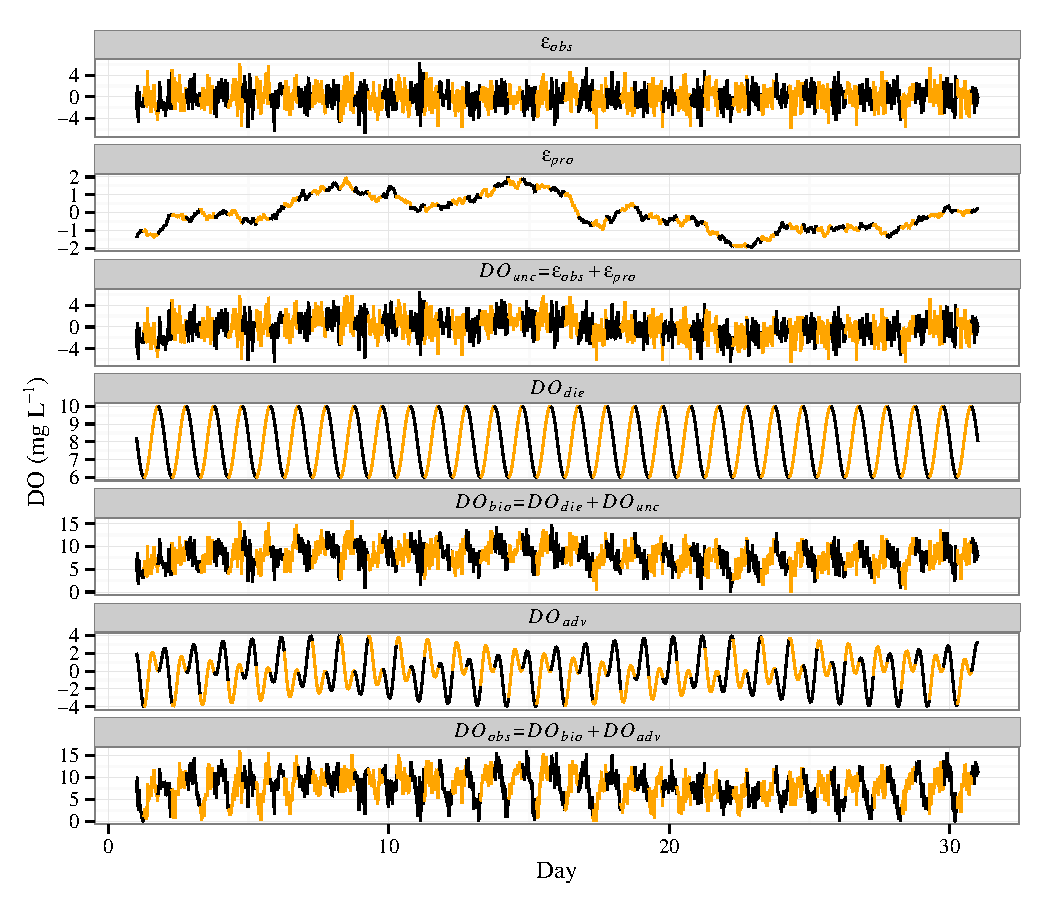
\includegraphics[width=\maxwidth]{figure/do_sim} 

}

\caption[Example of creating a simulated \ac{DO} time series]{Example of creating a simulated \ac{DO} time series.  Simulated values were estimated every thirty minutes for 31 days.  Yellow indicates daylight periods.\label{fig:do_sim}}
\end{figure}


\end{knitrout}
\vfill
\clearpage

% example of detiding a simulated time series
\centering\vspace*{\fill}
\begin{knitrout}
\definecolor{shadecolor}{rgb}{0.969, 0.969, 0.969}\color{fgcolor}\begin{kframe}


{\ttfamily\noindent\bfseries\color{errorcolor}{\#\# Error: could not find function "{}wtreg\_fun"{}}}

{\ttfamily\noindent\bfseries\color{errorcolor}{\#\# Error: object 'prd\_tmp' not found}}

{\ttfamily\noindent\bfseries\color{errorcolor}{\#\# Error: object 'prd\_tmp' not found}}

{\ttfamily\noindent\bfseries\color{errorcolor}{\#\# Error: it is only valid to get a child from a "{}gTree"{}}}\end{kframe}
\end{knitrout}
\vfill
\clearpage

% plot of representative time series for simulation
\centering\vspace*{\fill}
\begin{knitrout}
\definecolor{shadecolor}{rgb}{0.969, 0.969, 0.969}\color{fgcolor}\begin{figure}[!ht]


{\centering 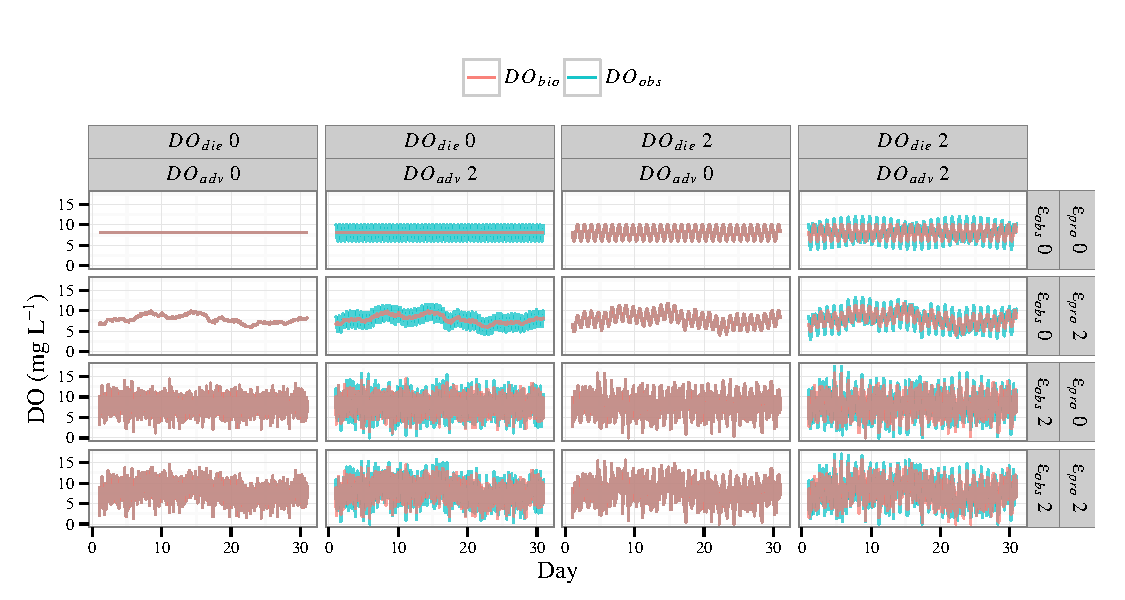
\includegraphics[width=\maxwidth]{figure/sim_ex} 

}

\caption[Representative examples of simulated \ac{DO} time series created by varying each of five parameters]{Representative examples of simulated \ac{DO} time series created by varying each of five parameters: tidal category (e.g., Mixed), strength of tidal association with \ac{DO} signal using $DO_{adv}$, amount of process uncertainty $\epsilon_{pro}$, amount of observation observation uncertainty $\epsilon_{obs}$, and strength of diel \ac{DO} component $DO_{die}$.  Parameter values represent the extremes used in the simulation (i.e., minimum, maximum).  Black lines are observed \ac{DO} from \cref{do_obs_all} and red lines are biological \ac{DO} from \cref{do_bio}.\label{fig:sim_ex}}
\end{figure}


\end{knitrout}
\vfill
\clearpage

% example of error surfaces 
\centering\vspace*{\fill}
\begin{knitrout}
\definecolor{shadecolor}{rgb}{0.969, 0.969, 0.969}\color{fgcolor}\begin{figure}[!ht]


{\centering 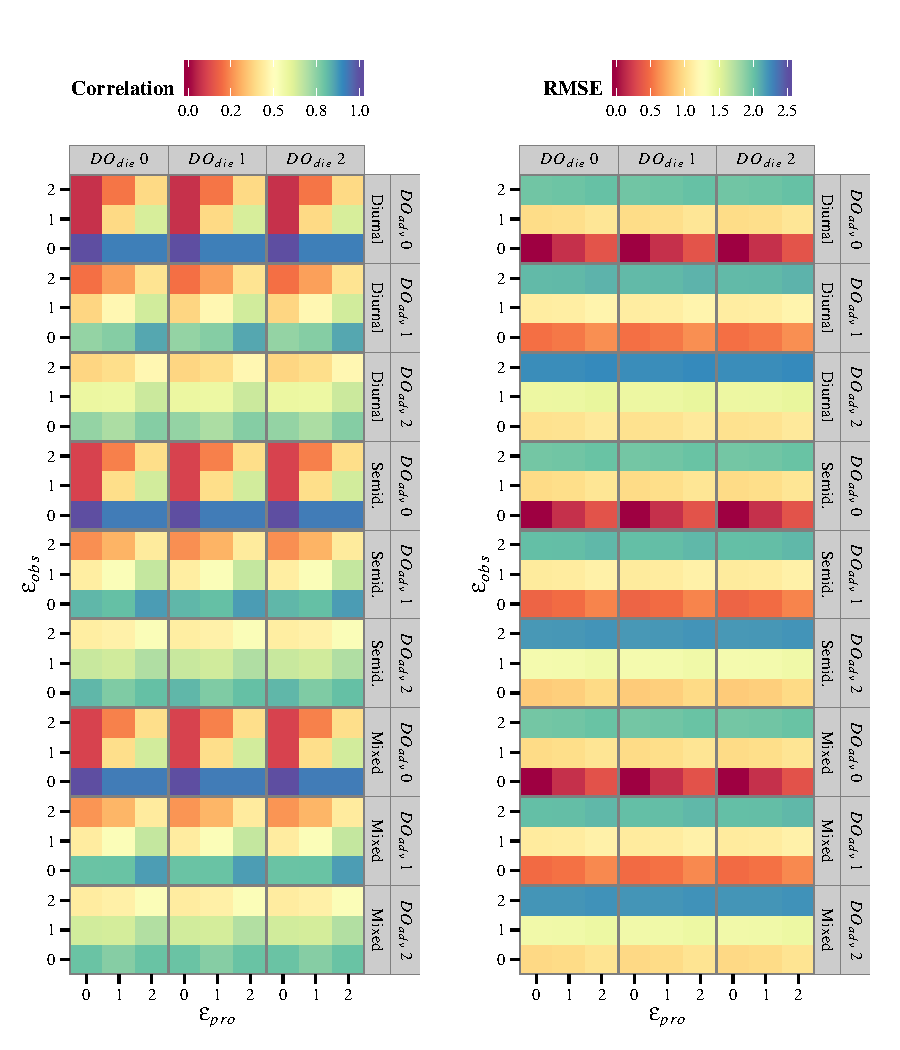
\includegraphics[width=\maxwidth]{figure/err_surf} 

}

\caption[Examples of correlations (left) and errors (right) between detided and biological \ac{DO} from weighted regression results]{Examples of correlations (left) and errors (right) between detided and biological \ac{DO} from weighted regression results.  Each tile represents a correlation or error value from results for a given combination of simulation parameters ($DO_{adv}$, $DO_{die}$, $\epsilon_{pro}$, $\epsilon_{obs}$) and selected window widths (two and ten days).  Results are for simulations using a diurnal tidal time series.\label{fig:err_surf}}
\end{figure}


\end{knitrout}
\vfill
\clearpage

% example of extreme scenario
\centering\vspace*{\fill}
\begin{knitrout}
\definecolor{shadecolor}{rgb}{0.969, 0.969, 0.969}\color{fgcolor}\begin{figure}[!ht]


{\centering 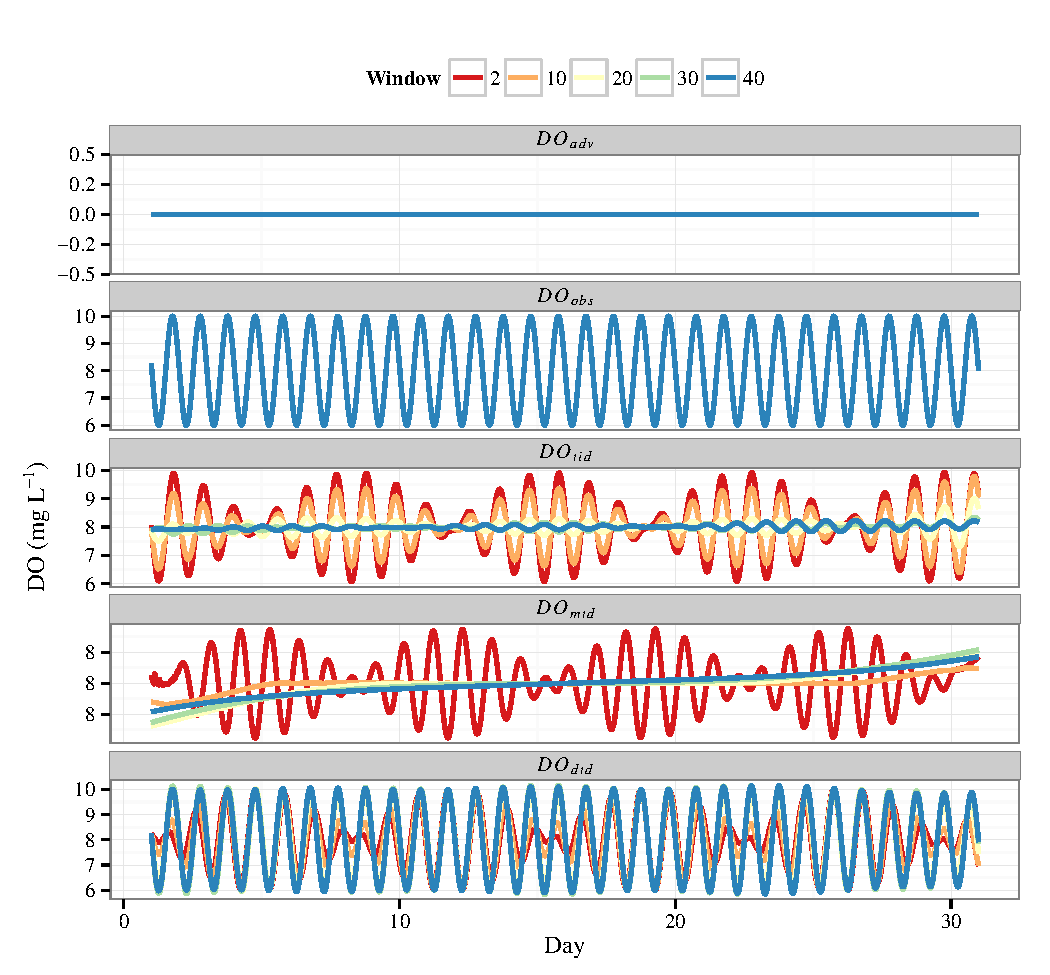
\includegraphics[width=\maxwidth]{figure/extreme} 

}

\caption[An extreme example of results from the weighted regression with decreasing window widths]{An extreme example of results from the weighted regression with decreasing window widths.  Results are for a simulated time series with a diurnal tidal component, no effect of tidal advection ($DO_{adv} = 0$), and an observed \ac{DO} signal dominated only by a diel component ($DO_{bio} = 2$, $\epsilon_{obs} = 0$, $\epsilon_{pro} = 0$).  Window widths varied form 2 to 40 days.  See \cref{do_tid,do_mtd,do_dtd,do_obs} for notation.\label{fig:extreme}}
\end{figure}


\end{knitrout}
\vfill
\clearpage

% maps of each case
\centering\vspace*{\fill}
\begin{knitrout}
\definecolor{shadecolor}{rgb}{0.969, 0.969, 0.969}\color{fgcolor}\begin{figure}[!ht]


{\centering 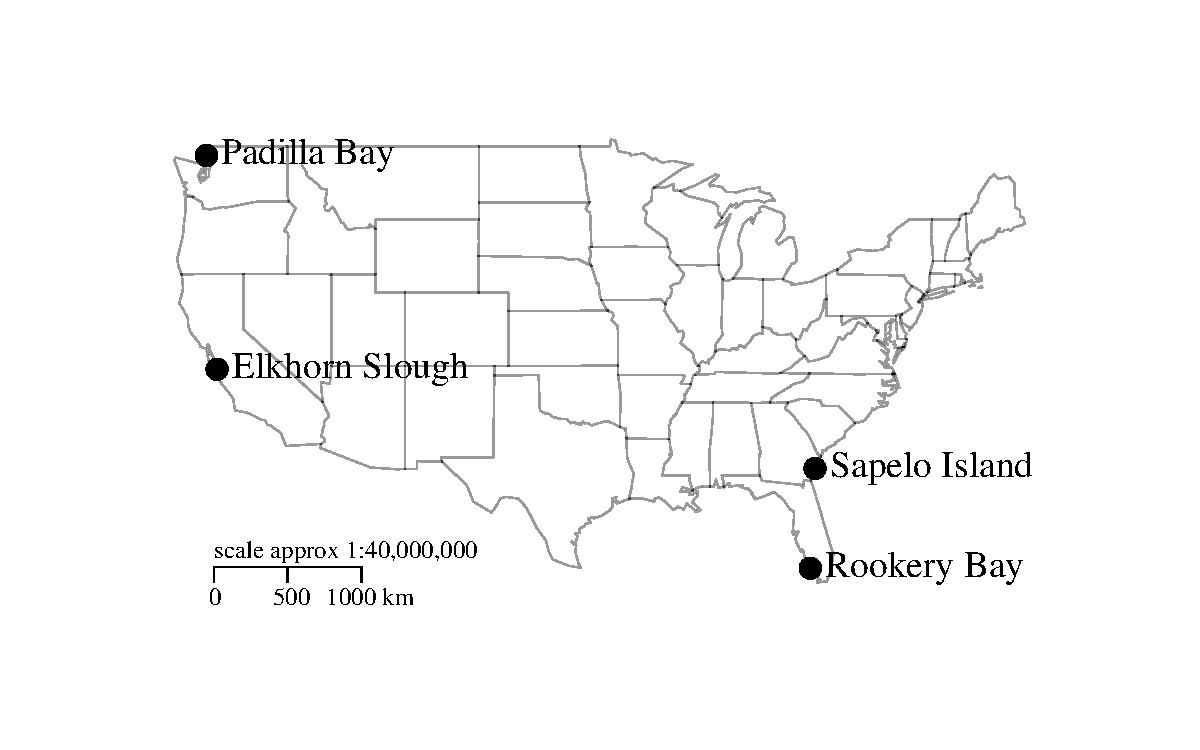
\includegraphics[width=\maxwidth]{figure/case_map} 

}

\caption[Locations of \ac{NERRS} sites used as case studies to evaluate of weighted regression]{Locations of \ac{NERRS} sites used as case studies to evaluate of weighted regression.  Individual stations at each reserve are PDBJE (Joe Leary Estuary at Padilla Bay), RKBMB (Middle Blackwater River at Rookery Bay), SAPDC (Dean Creek at Sapelo Island), and TJRBR (Boca Rio at Tijuana River).\label{fig:case_map}}
\end{figure}


\end{knitrout}
\vfill
\clearpage

% example from SAPDC
\centering\vspace*{\fill}
\begin{knitrout}
\definecolor{shadecolor}{rgb}{0.969, 0.969, 0.969}\color{fgcolor}\begin{kframe}


{\ttfamily\noindent\bfseries\color{errorcolor}{\#\# Error: do not know how to convert 'inst\_subs\$DateTimeStamp' to class "{}Date"{}}}

{\ttfamily\noindent\bfseries\color{errorcolor}{\#\# Error: 'names' attribute [1] must be the same length as the vector [0]}}

{\ttfamily\noindent\bfseries\color{errorcolor}{\#\# Error: object 'to\_plo1' not found}}

{\ttfamily\noindent\bfseries\color{errorcolor}{\#\# Error: object 'to\_plo1' not found}}

{\ttfamily\noindent\bfseries\color{errorcolor}{\#\# Error: object 'to\_plo1' not found}}

{\ttfamily\noindent\bfseries\color{errorcolor}{\#\# Error: object 'to\_plo1' not found}}

{\ttfamily\noindent\bfseries\color{errorcolor}{\#\# Error: object 'to\_plo1' not found}}

{\ttfamily\noindent\bfseries\color{errorcolor}{\#\# Error: do not know how to convert 'dat.in\$DateTimeStamp' to class "{}Date"{}}}

{\ttfamily\noindent\bfseries\color{errorcolor}{\#\# Error: object 'to\_plo2' not found}}

{\ttfamily\noindent\bfseries\color{errorcolor}{\#\# Error: object 'to\_plo2' not found}}

{\ttfamily\noindent\bfseries\color{errorcolor}{\#\# Error: object 'to\_plo2' not found}}

{\ttfamily\noindent\bfseries\color{errorcolor}{\#\# Error: do not know how to convert 'dat.in\$DateTimeStamp' to class "{}Date"{}}}

{\ttfamily\noindent\bfseries\color{errorcolor}{\#\# Error: object 'to\_plo2' not found}}

{\ttfamily\noindent\bfseries\color{errorcolor}{\#\# Error: object 'to\_plo2' not found}}

{\ttfamily\noindent\bfseries\color{errorcolor}{\#\# Error: object 'to\_plo3' not found}}\end{kframe}\begin{figure}[!ht]


{\centering 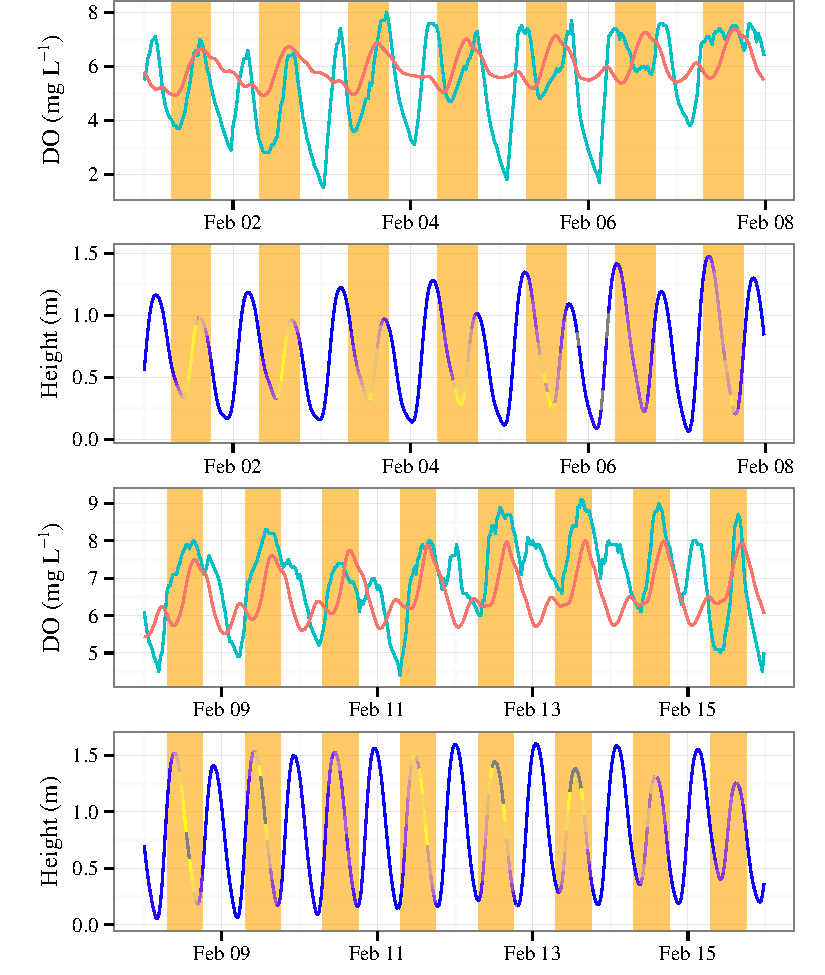
\includegraphics[width=0.8\textwidth]{figure/case_ex1} 

}

\caption[Example of metabolism and \ac{DO} time series before (observed) and after (detided) weighted regression]{Example of metabolism and \ac{DO} time series before (observed) and after (detided) weighted regression. Results are for a ten day period in March for the Sapelo Island station.\label{fig:case_ex1}}
\end{figure}


\end{knitrout}
\vfill
\clearpage

% example from ELKVM
\centering\vspace*{\fill}
\begin{knitrout}
\definecolor{shadecolor}{rgb}{0.969, 0.969, 0.969}\color{fgcolor}\begin{kframe}


{\ttfamily\noindent\bfseries\color{errorcolor}{\#\# Error: do not know how to convert 'inst\_subs\$DateTimeStamp' to class "{}Date"{}}}

{\ttfamily\noindent\bfseries\color{errorcolor}{\#\# Error: 'names' attribute [1] must be the same length as the vector [0]}}

{\ttfamily\noindent\bfseries\color{errorcolor}{\#\# Error: object 'to\_plo1' not found}}

{\ttfamily\noindent\bfseries\color{errorcolor}{\#\# Error: object 'to\_plo1' not found}}

{\ttfamily\noindent\bfseries\color{errorcolor}{\#\# Error: object 'to\_plo1' not found}}

{\ttfamily\noindent\bfseries\color{errorcolor}{\#\# Error: object 'to\_plo1' not found}}

{\ttfamily\noindent\bfseries\color{errorcolor}{\#\# Error: object 'to\_plo1' not found}}

{\ttfamily\noindent\bfseries\color{errorcolor}{\#\# Error: do not know how to convert 'dat.in\$DateTimeStamp' to class "{}Date"{}}}

{\ttfamily\noindent\bfseries\color{errorcolor}{\#\# Error: object 'to\_plo2' not found}}

{\ttfamily\noindent\bfseries\color{errorcolor}{\#\# Error: object 'to\_plo2' not found}}

{\ttfamily\noindent\bfseries\color{errorcolor}{\#\# Error: object 'to\_plo2' not found}}

{\ttfamily\noindent\bfseries\color{errorcolor}{\#\# Error: do not know how to convert 'dat.in\$DateTimeStamp' to class "{}Date"{}}}

{\ttfamily\noindent\bfseries\color{errorcolor}{\#\# Error: object 'to\_plo2' not found}}

{\ttfamily\noindent\bfseries\color{errorcolor}{\#\# Error: object 'to\_plo2' not found}}

{\ttfamily\noindent\bfseries\color{errorcolor}{\#\# Error: object 'to\_plo3' not found}}\end{kframe}\begin{figure}[!ht]


{\centering 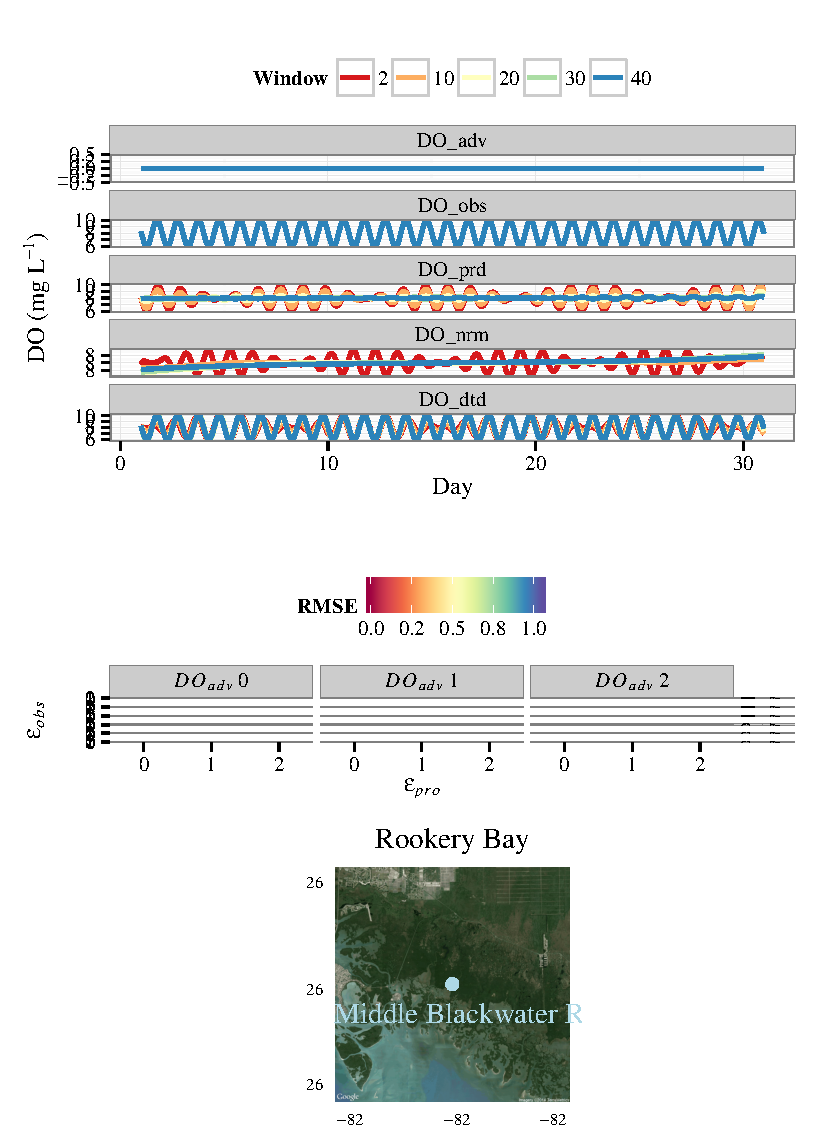
\includegraphics[width=0.8\textwidth]{figure/case_ex2} 

}

\caption[Example of metabolism and \ac{DO} time series before (observed) and after (detided) weighted regression]{Example of metabolism and \ac{DO} time series before (observed) and after (detided) weighted regression. Results are for a ten day period in March for the Elkhorn Slough station.\label{fig:case_ex2}}
\end{figure}


\end{knitrout}
\vfill
\clearpage

% example from pdbby
\centering\vspace*{\fill}
\begin{knitrout}
\definecolor{shadecolor}{rgb}{0.969, 0.969, 0.969}\color{fgcolor}\begin{kframe}


{\ttfamily\noindent\bfseries\color{errorcolor}{\#\# Error: do not know how to convert 'inst\_subs\$DateTimeStamp' to class "{}Date"{}}}

{\ttfamily\noindent\bfseries\color{errorcolor}{\#\# Error: 'names' attribute [1] must be the same length as the vector [0]}}

{\ttfamily\noindent\bfseries\color{errorcolor}{\#\# Error: object 'to\_plo1' not found}}

{\ttfamily\noindent\bfseries\color{errorcolor}{\#\# Error: object 'to\_plo1' not found}}

{\ttfamily\noindent\bfseries\color{errorcolor}{\#\# Error: object 'to\_plo1' not found}}

{\ttfamily\noindent\bfseries\color{errorcolor}{\#\# Error: object 'to\_plo1' not found}}

{\ttfamily\noindent\bfseries\color{errorcolor}{\#\# Error: object 'to\_plo1' not found}}

{\ttfamily\noindent\bfseries\color{errorcolor}{\#\# Error: do not know how to convert 'dat.in\$DateTimeStamp' to class "{}Date"{}}}

{\ttfamily\noindent\bfseries\color{errorcolor}{\#\# Error: object 'to\_plo2' not found}}

{\ttfamily\noindent\bfseries\color{errorcolor}{\#\# Error: object 'to\_plo2' not found}}

{\ttfamily\noindent\bfseries\color{errorcolor}{\#\# Error: object 'to\_plo2' not found}}

{\ttfamily\noindent\bfseries\color{errorcolor}{\#\# Error: do not know how to convert 'dat.in\$DateTimeStamp' to class "{}Date"{}}}

{\ttfamily\noindent\bfseries\color{errorcolor}{\#\# Error: object 'to\_plo2' not found}}

{\ttfamily\noindent\bfseries\color{errorcolor}{\#\# Error: object 'to\_plo2' not found}}

{\ttfamily\noindent\bfseries\color{errorcolor}{\#\# Error: object 'to\_plo3' not found}}\end{kframe}\begin{figure}[!ht]


{\centering 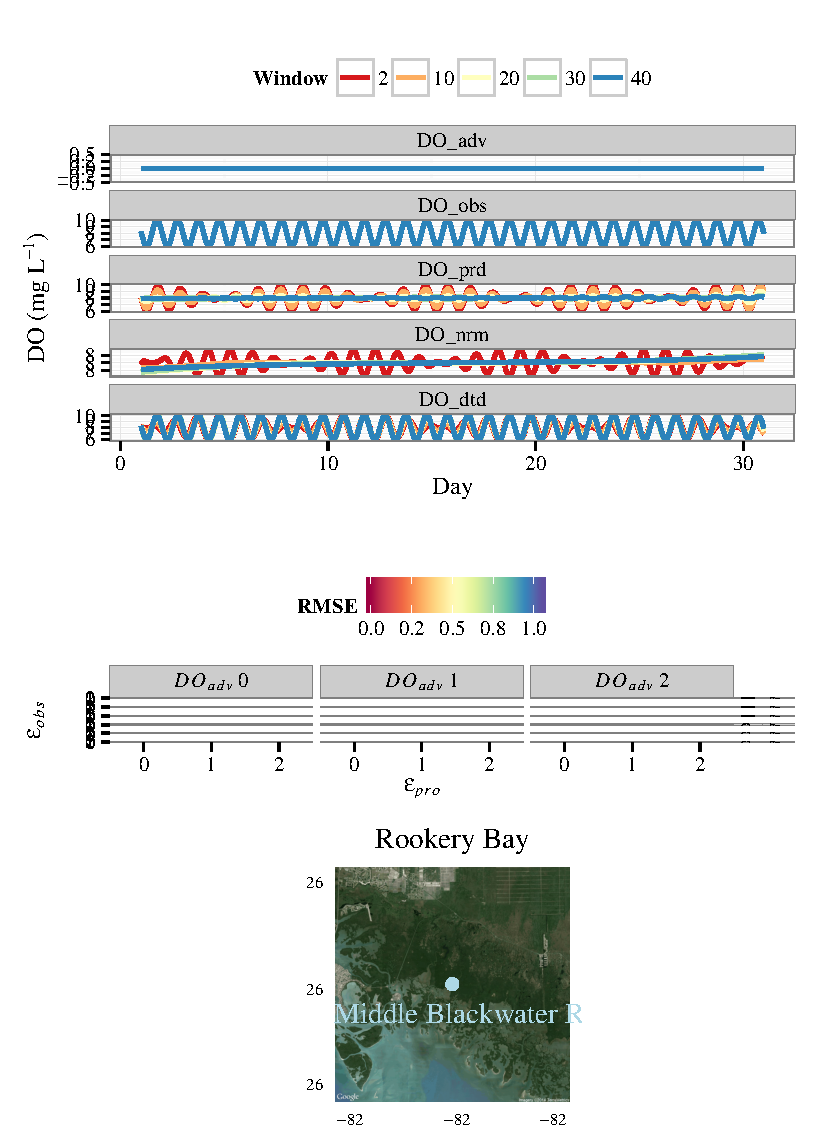
\includegraphics[width=0.8\textwidth]{figure/case_ex3} 

}

\caption[Example of metabolism and \ac{DO} time series before (observed) and after (detided) weighted regression]{Example of metabolism and \ac{DO} time series before (observed) and after (detided) weighted regression. Results are for a ten day period in March for the Padilla Bay station.\label{fig:case_ex3}}
\end{figure}


\end{knitrout}
\vfill
\clearpage

%%%%%%
% tables

% summary of simulation performance for detided and biological
% latex.default(tab, file = "", rowlabel = "Parameter", caption = cap.val,      caption.loc = "top", rgroup = Parms, n.rgroup = c(rep(3,          5), 5), cgroup = c("Correlation", "RMSE"), n.cgroup = c(2,          2), rowname = rows, colheads = rep(c("Mean", "Std. Err."),          2), label = "tab:dtd_perf") 
%
\begin{table}[!tbp]
\caption{Mean correlations and error estimates between detided and biological \ac{DO} time series for different simulation parameters (tidal category, $DO_{die}$, $DO_{adv}$, $\epsilon_{pro}$, $\epsilon_{obs}$) and window widths (days).  Each value represents a combination of results from multiple simulations with the parameter value held constant for each row (e.g., row one is a summary of all simulations for which the tidal category was diurnal).\label{tab:dtd_perf}} 
\begin{center}
\begin{tabular}{lllcll}
\hline\hline
\multicolumn{1}{l}{\bfseries Parameter}&\multicolumn{2}{c}{\bfseries Correlation}&\multicolumn{1}{c}{\bfseries }&\multicolumn{2}{c}{\bfseries RMSE}\tabularnewline
\cline{2-3} \cline{5-6}
\multicolumn{1}{l}{}&\multicolumn{1}{c}{Mean}&\multicolumn{1}{c}{Std. Err.}&\multicolumn{1}{c}{}&\multicolumn{1}{c}{Mean}&\multicolumn{1}{c}{Std. Err.}\tabularnewline
\hline
{\bfseries Tidal category}&&&&&\tabularnewline
~~Diurnal&0.97&0.02&&0.24&0.09\tabularnewline
~~Semidiurnal&1.00&0.00&&0.07&0.02\tabularnewline
~~Mixed Semidiurnal&0.99&0.01&&0.18&0.07\tabularnewline
\hline
{\bfseries $\boldsymbol{DO_{die}}$}&&&&&\tabularnewline
~~0&1.00&0.00&&0.07&0.02\tabularnewline
~~1&0.98&0.01&&0.15&0.05\tabularnewline
~~2&0.97&0.02&&0.27&0.10\tabularnewline
\hline
{\bfseries $\boldsymbol{DO_{adv}}$}&&&&&\tabularnewline
~~0&0.99&0.01&&0.16&0.07\tabularnewline
~~1&0.99&0.01&&0.16&0.07\tabularnewline
~~2&0.99&0.01&&0.16&0.07\tabularnewline
\hline
{\bfseries $\boldsymbol{\epsilon_{pro}}$}&&&&&\tabularnewline
~~0&0.98&0.02&&0.16&0.07\tabularnewline
~~1&0.98&0.01&&0.16&0.07\tabularnewline
~~2&0.99&0.01&&0.17&0.07\tabularnewline
\hline
{\bfseries $\boldsymbol{\epsilon_{obs}}$}&&&&&\tabularnewline
~~0&0.98&0.02&&0.13&0.07\tabularnewline
~~1&0.99&0.01&&0.16&0.07\tabularnewline
~~2&0.99&0.01&&0.21&0.07\tabularnewline
\hline
{\bfseries Window}&&&&&\tabularnewline
~~2&0.95&0.02&&0.38&0.10\tabularnewline
~~10&0.98&0.01&&0.24&0.08\tabularnewline
~~20&1.00&0.00&&0.09&0.02\tabularnewline
~~30&1.00&0.00&&0.05&0.01\tabularnewline
~~40&1.00&0.00&&0.04&0.01\tabularnewline
\hline
\end{tabular}
\end{center}
\end{table}



% descriptive table of case studies
% latex.default(tab, file = "", rowlabel = "Site", insert.bottom = foot.val,      caption = cap.val, caption.loc = "top", cgroup = c("Tidal amplitude",          "DO", "Metabolism\\textsuperscript{\\textit{a}}"), n.cgroup = c(4,          2, 3), rowname = rows, colheads = c("O1", "P1", "M2",          "S2", "Range", "Mean", "Pg", "Rt", "NEM"), label = "tab:case_att") 
%
\begin{table}[!tbp]
\caption{Summary statistics of tidal component amplitudes (m), \ac{DO} (mg L$^{-1}$), and metabolism estimates (gross production, respiration, and net ecosystem metabolism as g m$^{-2}$ d$^{-1}$) for each case study.  Tidal components are principal lunar semidiurnal (O1, frequency 25.82 hours), solar diurnal (P1, 24.07 hours), lunar semidiurnal (M2, 12.42 hours), and solar semidiurnal (S2, 12 hours), estimated from harmonic regressions of tidal height (\texttt{oce} package in R, \citealt{Foreman89}, \citetalias{RDCT14}).  \ac{DO} range and mean are grand means of daily estimates for the entire period of record (30 minute observations) for each site.  Metabolism estimates are means of daily integrated values.\label{tab:case_att}} 
\begin{center}
\begin{tabular}{lllllcllclll}
\hline\hline
\multicolumn{1}{l}{\bfseries Site}&\multicolumn{4}{c}{\bfseries Tidal amplitude}&\multicolumn{1}{c}{\bfseries }&\multicolumn{2}{c}{\bfseries DO}&\multicolumn{1}{c}{\bfseries }&\multicolumn{3}{c}{\bfseries Metabolism\textsuperscript{\textit{a}}}\tabularnewline
\cline{2-5} \cline{7-8} \cline{10-12}
\multicolumn{1}{l}{}&\multicolumn{1}{c}{O1}&\multicolumn{1}{c}{P1}&\multicolumn{1}{c}{M2}&\multicolumn{1}{c}{S2}&\multicolumn{1}{c}{}&\multicolumn{1}{c}{Range}&\multicolumn{1}{c}{Mean}&\multicolumn{1}{c}{}&\multicolumn{1}{c}{Pg}&\multicolumn{1}{c}{Rt}&\multicolumn{1}{c}{NEM}\tabularnewline
\hline
ELKVM&0.24&0.12&0.48&0.13&&6.79&7.86&&5.42&-8.58&-3.16\tabularnewline
PDBBY&0.46&0.23&0.63&0.15&&7.53&8.97&&8.03&-8.59&-0.56\tabularnewline
RKBMB&0.13&0.04&0.36&0.10&&5.47&4.53&&2.46&-3.24&-0.78\tabularnewline
SAPDC&0.10&0.02&0.54&0.07&&7.98&5.01&&4.46&-6.37&-1.90\tabularnewline
\hline
\end{tabular}
\end{center}
\footnotesize\textsuperscript{\textit{a}}Pg: gross production, Rt: respiration, NEM: net ecosystem metabolism\end{table}



% correlations with tide before/after wtreg
% latex.default(tab, file = "", rowlabel = "Site", rgroup = unique(rows),      n.rgroup = rep(2, 4), insert.bottom = foot.val, caption = cap.val,      colheads = c("DO", "DO flux", "Pg\\textsuperscript{\\textit{a}}",          "Rt", "NEM"), caption.loc = "top", rowname = rep(c("Observed",          "Detided"), 4), label = "tab:cor_res") 
%
\begin{table}[!tbp]
\caption{Correlations of tidal changes at each site with continuous \ac{DO} observations, instantaneous \ac{DO} flux, and metabolism estimates (gross production, respiration, and net metabolism) before (observed) and after detiding with weighted regression.  \ac{DO} values are correlated with predicated tidal height at each observation, \ac{DO} flux values are correlated with tidal change between observations, and daily integrated metabolism estimates are correlated with daily tidal range.\label{tab:cor_res}} 
\begin{center}
\begin{tabular}{llllll}
\hline\hline
\multicolumn{1}{l}{Site}&\multicolumn{1}{c}{DO}&\multicolumn{1}{c}{DO flux}&\multicolumn{1}{c}{Pg\textsuperscript{\textit{a}}}&\multicolumn{1}{c}{Rt}&\multicolumn{1}{c}{NEM}\tabularnewline
\hline
{\bfseries ELKVM}&&&&&\tabularnewline
~~Observed& 0.48***& 0.26***& 0.05 & 0.00 & 0.08 \tabularnewline
~~Detided& 0.01 &-0.04***&-0.01 & 0.06 & 0.07 \tabularnewline
\hline
{\bfseries PDBBY}&&&&&\tabularnewline
~~Observed&-0.45***&-0.31***&-0.12*& 0.03 &-0.10 \tabularnewline
~~Detided& 0.00 & 0.02**& 0.08 &-0.17**&-0.12*\tabularnewline
\hline
{\bfseries RKBMB}&&&&&\tabularnewline
~~Observed& 0.28***& 0.39***& 0.03 & 0.09 & 0.21***\tabularnewline
~~Detided&-0.01 & 0.02*&-0.08 & 0.16**& 0.18**\tabularnewline
\hline
{\bfseries SAPDC}&&&&&\tabularnewline
~~Observed& 0.48***& 0.62***&-0.02 & 0.00 &-0.04 \tabularnewline
~~Detided&-0.01 &-0.04***&-0.04 &-0.03 &-0.10*\tabularnewline
\hline
\end{tabular}
\end{center}
\footnotesize *$p<0.05$; **$p<0.01$; ***$p<0.001$\\\textsuperscript{\textit{a}}Pg: gross production, Rt: respiration, NEM: net ecosystem metabolism\end{table}



% case study metabolism results, including perc anom
% latex.default(tab, file = "", rowlabel = "Site", insert.bottom = foot.val,      caption = cap.val, caption.loc = "top", rgroup = gsub("_wtreg.RData",          "", unique(to_tab$Site)), n.rgroup = rep(2, 4), cgroup = c("Pg\\textsuperscript{\\textit{a}}",          "Rt", "NEM"), n.cgroup = c(3, 3, 2), rowname = rows,      colheads = c(rep(c("Mean", "Std. Err.", "Anom"), 2), c("Mean",          "Std. Err.")), label = "tab:case_res") 
%
\begin{table}[!tbp]
\caption{Metabolism estimates (gross production, respiration, and net metabolism) for case studies using \ac{DO} time series before (observed) and after (detided) application of weighted regression.  Means and standard errors are based on daily integrated metabolism estimates.  Anomalous values are the proportion of metabolism estimates that were negative for gross production and positive for respiration.\label{tab:case_res}} 
\begin{center}
\begin{tabular}{llllclllcll}
\hline\hline
\multicolumn{1}{l}{\bfseries Site}&\multicolumn{3}{c}{\bfseries Pg\textsuperscript{\textit{a}}}&\multicolumn{1}{c}{\bfseries }&\multicolumn{3}{c}{\bfseries Rt}&\multicolumn{1}{c}{\bfseries }&\multicolumn{2}{c}{\bfseries NEM}\tabularnewline
\cline{2-4} \cline{6-8} \cline{10-11}
\multicolumn{1}{l}{}&\multicolumn{1}{c}{Mean}&\multicolumn{1}{c}{Std. Err.}&\multicolumn{1}{c}{Anom}&\multicolumn{1}{c}{}&\multicolumn{1}{c}{Mean}&\multicolumn{1}{c}{Std. Err.}&\multicolumn{1}{c}{Anom}&\multicolumn{1}{c}{}&\multicolumn{1}{c}{Mean}&\multicolumn{1}{c}{Std. Err.}\tabularnewline
\hline
{\bfseries ELKVM}&&&&&&&&&&\tabularnewline
~~Observed&5.42&0.70&0.28&&-8.58&0.78&0.23&&-3.16&0.40\tabularnewline
~~Detided&0.02&0.54&0.39&&-2.47&0.51&0.33&&-2.45&0.37\tabularnewline
\hline
{\bfseries PDBBY}&&&&&&&&&&\tabularnewline
~~Observed&8.03&0.70&0.20&&-8.59&0.78&0.16&&-0.56&0.57\tabularnewline
~~Detided&6.31&0.65&0.22&&-6.97&0.67&0.24&&-0.66&0.49\tabularnewline
\hline
{\bfseries RKBMB}&&&&&&&&&&\tabularnewline
~~Observed&2.46&0.14&0.14&&-3.24&0.16&0.10&&-0.78&0.09\tabularnewline
~~Detided&2.59&0.12&0.11&&-3.28&0.15&0.09&&-0.69&0.08\tabularnewline
\hline
{\bfseries SAPDC}&&&&&&&&&&\tabularnewline
~~Observed&4.46&0.25&0.17&&-6.37&0.27&0.11&&-1.90&0.15\tabularnewline
~~Detided&4.48&0.17&0.09&&-6.12&0.20&0.05&&-1.65&0.12\tabularnewline
\hline
\end{tabular}
\end{center}
\textsuperscript{\textit{a}}Pg: gross production, Rt: respiration, NEM: net ecosystem metabolism\end{table}



\end{document}
